% Profile / signal transformer decoder.  Build: latexmk -pdf transformer.tex
\documentclass[border=8pt]{standalone}
\usepackage{amsmath}
% Shared TikZ palette + node styles for the ML-RT2 architecture diagrams.
% Colours match the ML-RT comparison-paper figures so the three papers look consistent:
%   pink   = data / vectors (inputs, outputs, latent representations)
%   blue   = learned networks / operators (MLPs, encoders, decoders, ...)
%   orange = special operations / physics (spectral transforms, RT residual, ...)
%   green  = loss / training terms
\usepackage{tikz}
\usetikzlibrary{arrows.meta,positioning,fit,backgrounds,calc}

\definecolor{dataFill}{HTML}{F2E6FF}\definecolor{dataDraw}{HTML}{6600CC}
\definecolor{netFill}{HTML}{B5E8E8}\definecolor{netDraw}{HTML}{086565}
\definecolor{opFill}{HTML}{FFE0C2}\definecolor{opDraw}{HTML}{AB4F03}
\definecolor{lossFill}{HTML}{C8F4C1}\definecolor{lossDraw}{HTML}{0C5600}

\tikzset{
  font=\small,
  box/.style  ={draw, rounded corners, align=center, inner sep=4pt, minimum height=9mm, line width=0.3mm},
  data/.style ={box, fill=dataFill, draw=dataDraw},
  net/.style  ={box, fill=netFill,  draw=netDraw},
  op/.style   ={box, fill=opFill,   draw=opDraw},
  loss/.style ={box, fill=lossFill, draw=lossDraw},
  sum/.style  ={draw=netDraw, circle, inner sep=1.3pt, fill=white, line width=0.3mm},
  arr/.style  ={-{Stealth[length=2.4mm]}, thick},
  darr/.style ={-{Stealth[length=2.4mm]}, thick, dashed},
  note/.style ={align=center, font=\scriptsize, text=black!65},
}

\begin{document}
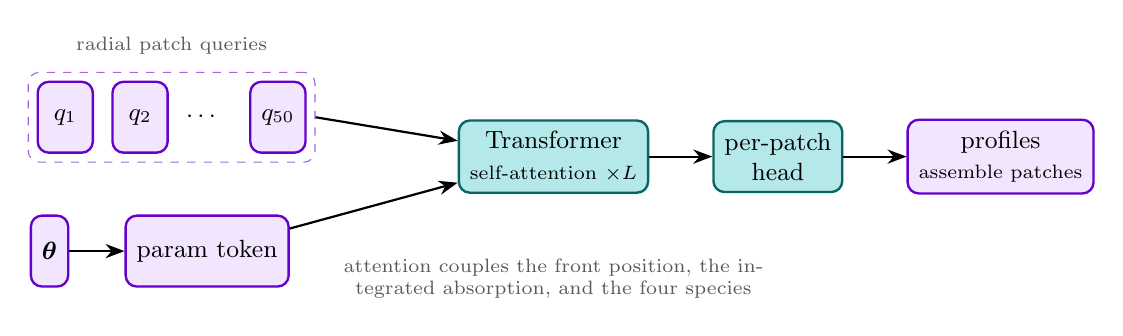
\begin{tikzpicture}
  % query tokens, grouped in a dashed box with a single arrow out (no lines through boxes)
  \node[data, minimum width=7mm] (q1) at (0,0)      {$q_1$};
  \node[data, minimum width=7mm] (q2) at (0.95,0)   {$q_2$};
  \node                          (qd) at (1.75,0)   {$\cdots$};
  \node[data, minimum width=7mm] (qn) at (2.7,0)    {$q_{50}$};
  \begin{scope}[on background layer]
    \node[draw=dataDraw!60, dashed, rounded corners, inner sep=3pt,
          fit=(q1)(q2)(qd)(qn)] (qbox) {};
  \end{scope}
  \node[note, above=1mm of qbox] {radial patch queries};

  % parameter token (below), and the main flow
  \node[data] (th) at (-0.2,-1.7) {$\boldsymbol{\theta}$};
  \node[data, minimum width=12mm, right=7mm of th] (pt) {param token};
  \node[net,  minimum width=22mm] (enc)  at (6.2,-0.5) {Transformer\\{\scriptsize self-attention $\times L$}};
  \node[net,  right=8mm of enc]   (head) {per-patch\\head};
  \node[data, right=8mm of head]  (out)  {profiles\\{\scriptsize assemble patches}};

  \draw[arr] (th) -- (pt);
  \draw[arr] (qbox.east) -- (enc);
  \draw[arr] (pt) -- (enc);
  \draw[arr] (enc) -- (head);  \draw[arr] (head) -- (out);
  \node[note, text width=70mm, below=7mm of enc]
        {attention couples the front position, the integrated absorption, and the four species};
\end{tikzpicture}
\end{document}
